\subsection{Integration in die UH Codebase}
\subsubsection{Das Kartenformat}
\label{kartenformat}

%
% algorithm principle
%
\begin{figure}[htbp]
  \centering
  
    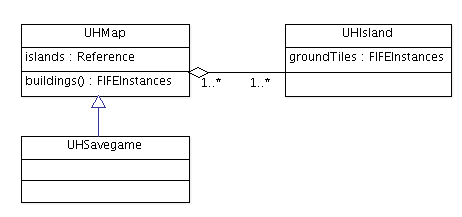
\includegraphics[width=0.7\textwidth]{gfx/klassendiagramm-UHSaveGame.png}
  
  \caption{UML Diagramm des Kartenformates von UH.}
  \label{figure:automaton-intersection}
\end{figure}

UHs Kartenformat im SQLite besteht grob aus den folgenden Elementen für den
Editor relevanten Elementen:
\begin{itemize}
  \item Allgemeinen Karteninformationen
  \item Die auf der Karte plazierten Objekte (wie Gebäude etc.)
  \item Verweise auf Island-Files. \\ 
  Ein Island-File ist eine SQLite-Datenbank,
  die die Informationen über die Bodenbeschaffenheit einer zusammengehörenden
  Inseln enthält:
  \begin{itemize}
    \item Allgemeine Islandinformationen
    \item Alle zu einem Island gehörenden Groundtiles
  \end{itemize}
\end{itemize} 

\subsection{Kommandozeilen-Parameter (FIFE)}
\subsection{Schaffung der Plugin-Infrastruktur (FIFE)}

\subsection{Plugin zum Laden von UH Objekten (UH)}
\subsection{Plugin zum Laden von UH Karten (UH)}
\subsection{Plugin zum Speichern von UH Karten (UH)}
Das Plugin zum Speichern weist die Schwierigkeit auf, dass der Editor nicht die
Interna des UH Spielmodells kennen kann. Der Editor ``zeichnet'' einfach nur
Elemente wie Bodentiles und Gebäude auf die verschiedenen Layer-Schichten, das
Saver-Plugin muss diese im UH-Modell speichern. 


Die Layer-Schichten enthalten vor dem Speichern die Instanzen aller vom User
gesetzen Gebäude und Bodentiles. 

Der Algorithmus geht dabei den Groundlayer vom Urpsrung des Koordinatensystems
Origo (0, 0) nach rechts unten ab. Durch diese Traversierungsstrategie muss nur
nach oben und nach links auf zu verbindenden Islands überprüft werden. Findet
sich ein direkt angrenzendes Groundtiles, so wird das akutelle Groundtiles (rot
hinterlegt) mit dem bestehenden vereinigt, indem es dessen Insel-ID übernimmt.

%
% algorithm principle
%
\begin{figure}[htbp]
  \centering
  
    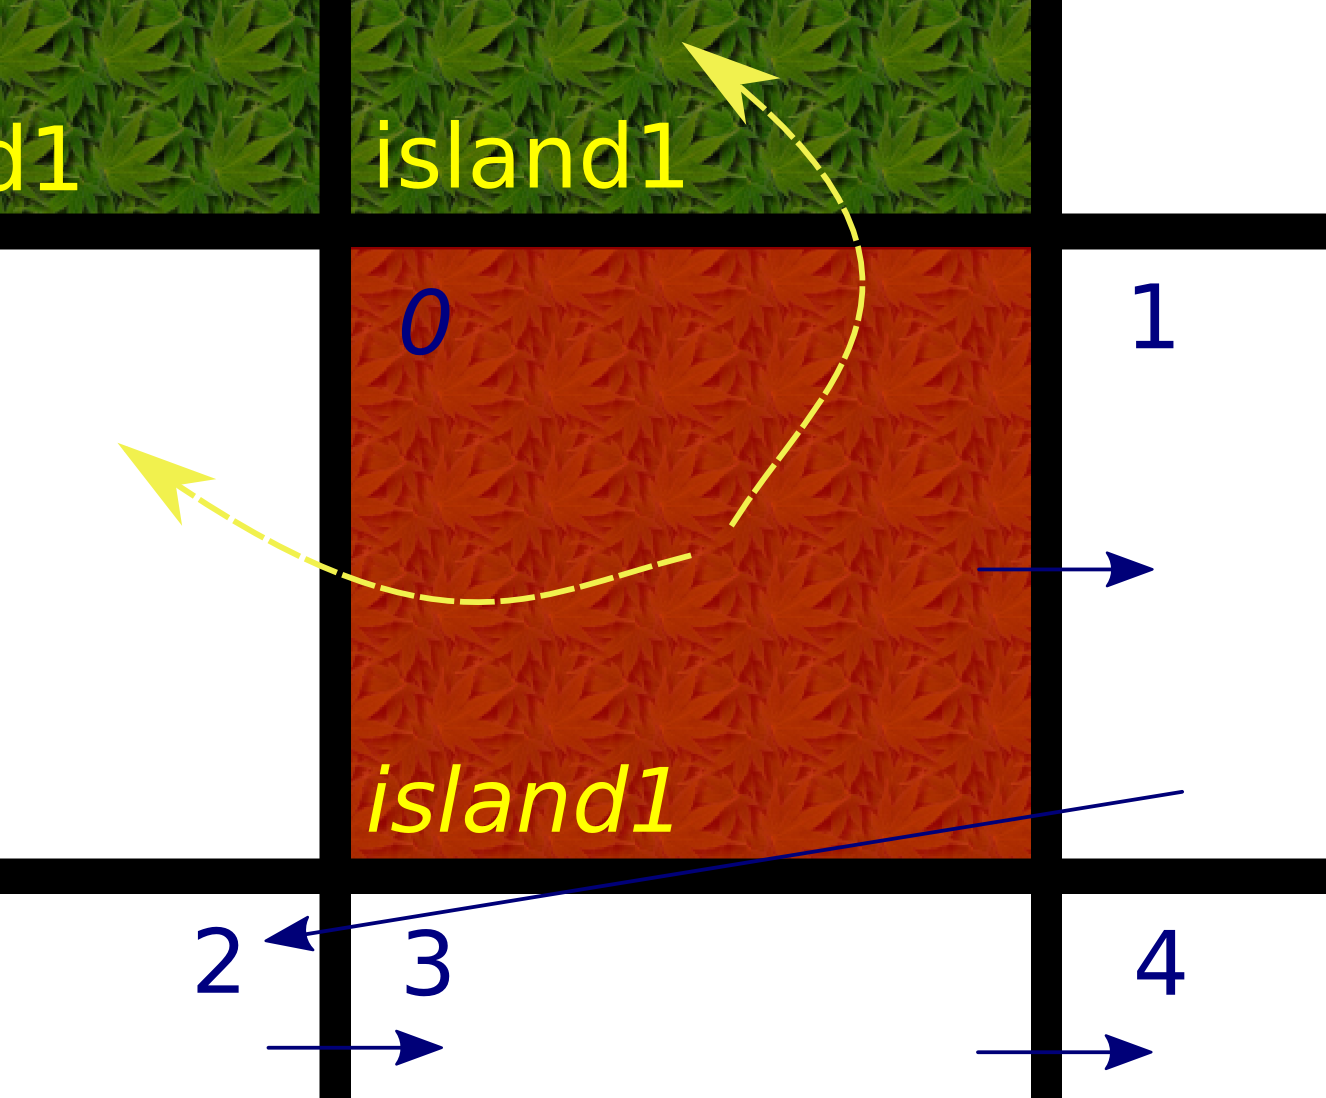
\includegraphics[width=0.7\textwidth]{gfx/merge_algorithm.png}
  
  \caption{Der Partitionierungsalgorithmus für die Islands. Die gelben Pfeile
  geben an, welche Gitterflächen auf das Vorhandensein von Tiles überprüft
  werden. Der Algorithmus traversiert die Tiles von oben links nach unten
  rechts (blau eingezeichnet).}
  \label{figure:automaton-intersection}
\end{figure}

Wie in Abschnitt \ref{kartenformat} erklärt, besteht die Schwierigkeit des
Transformationsprozesses in diese Richtung darin, zusammenliegende Bodentiles zu
erkennen. Dadurch benötigt das Speichern großer Inseln eine gewisse Zeit bis die
Gruppierung der Inslen beendet ist.
